\documentclass[aspectratio=169]{beamer}

\usetheme{nestlab}

\title{Sample presentation}
\subtitle{This is a subtitle}
\author{Firstname Lastname}
\institute{Worcester Polytechnic Institute}
\date{\today}

\begin{document}

\maketitle

\section{Section example}

\begin{frame}
  \frametitle{Lists}
  \begin{itemize}
  \item One
    \begin{itemize}
    \item Two
      \begin{itemize}
      \item Three
      \end{itemize}
    \end{itemize}
  \end{itemize}

  \begin{enumerate}
  \item One
    \begin{enumerate}
    \item Two
      \begin{enumerate}
      \item Three
      \end{enumerate}
    \end{enumerate}
  \end{enumerate}

  \begin{description}[One]
  \item[One] One
    \begin{description}[Two]
    \item[Two] Two
      \begin{description}[Three]
      \item[Three] Three
      \end{description}
    \end{description}
  \end{description}
\end{frame}

\begin{frame}
  \frametitle{Text blocks}
  
  \begin{block}{Block title}
    Block content
  \end{block}

  \begin{exampleblock}{Example title}
    Example content
  \end{exampleblock}

  \begin{example}[Example title]
    Example content
  \end{example}

  \begin{theorem}[Theorem title]
    Theorem content
  \end{theorem}

  \begin{definition}[Definition title]
    Definition content
  \end{definition}
\end{frame}

\begin{frame}
  \frametitle{Math example}
  \begin{equation}
    e^x = \lim_{n \to \infty}\left(1 + \frac{x}{n}\right)^n
  \end{equation}
\end{frame}

\begin{citeframe}{Author}{Title}{Venue, Year}
  \frametitle{Citation example}
\end{citeframe}

\begin{frame}
  \frametitle{Graphics example}
  \centering
  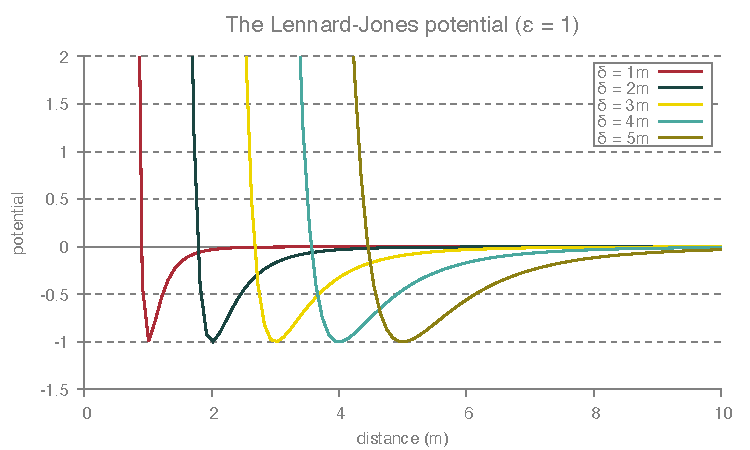
\includegraphics{plot}
\end{frame}

\end{document}